%%%%%%%%%%%%%%%%%%%%%%%%%%%%%%%%%%%%%%%%%%%%%%%%%%%%%%%%%%%%%%%%%%%%%%%%%%%%%%%%%%%%%
%																					%
%	TRABAJO: Proyecto Integrador													%
%																					%
%		Titulo: 	Desarrollo de IP cores con procesamiento de Redes de Petri 		%
%					Temporales para sistemas multicore en FPGA						%
%																					%
%		Autores:	Juli�n Nonino													%
%					Carlos Renzo Pisetta											%
%					Orlando Micolini												%
%																					%
%	Parte: Apendices																%
%	Capitulo: Interrupciones en los IP core											%
%	Archivo: interrupciones.tex														%
%																					%
%%%%%%%%%%%%%%%%%%%%%%%%%%%%%%%%%%%%%%%%%%%%%%%%%%%%%%%%%%%%%%%%%%%%%%%%%%%%%%%%%%%%%

% Path Imagenes: ./apendices/interrupciones/img
% Nombre predeterminado imagenes: intxx
%	xx es el numero de imagen

\chapter{Interrupciones en los IP cores}
	\label{ap:interrupciones}

	Para poder aprovechar las ventajas del uso de interrupciones en sistemas que utilizan el bus AXI, es 
	necesario usar un controlador de interrupciones llamado \textbf{$axi_inc$}. Este IP core se conecta al bus 
	y a los distintos IP cores que generan interrupciones y los dirige estas se�ales hacia el procesador, en 
	este caso un MicroBlaze.

	Las interrupciones puedes ser por nivel o flanco, pero una vez que se elige alguna de estas opciones, se 
	debe respetar en todos los IP cores que se encuentren conectados a un mismo controlador de interrupciones. 

	Si el sistema que se est� creando con el XPS es un sistema que utiliza el bus PLB\footnotemark , el 
	asistente de creaci�n de nuevos IP cores posibilita que el desarrollador indique que el IP core que esta 
	creando generar� interrupciones.
	\footnotetext{$http://www.xilinx.com/support/documentation/ip_documentation/plb_v46.pdf$}
	En sistemas AXI, el desarrollador debe generar un IP core como se detalla en el Apendice 
	\ref{ap:creacion_IP_core}:Creaci�n de un nuevo IP core
	y luego agregar elementos tanto el hardware como el software para dar soporte a las interrupciones.
\newpage
	
	\section{Modificaciones en el Hardware}
		Para comenzar en el archivo ``user\_logic.v'' del IP core se debe declarar un puerto de salida que ser� 
		la se�al de interrupci�n generada por el IP core(Figura\ref{fig:int01}).
		
			\begin{figure}[H]
				\begin{center}
					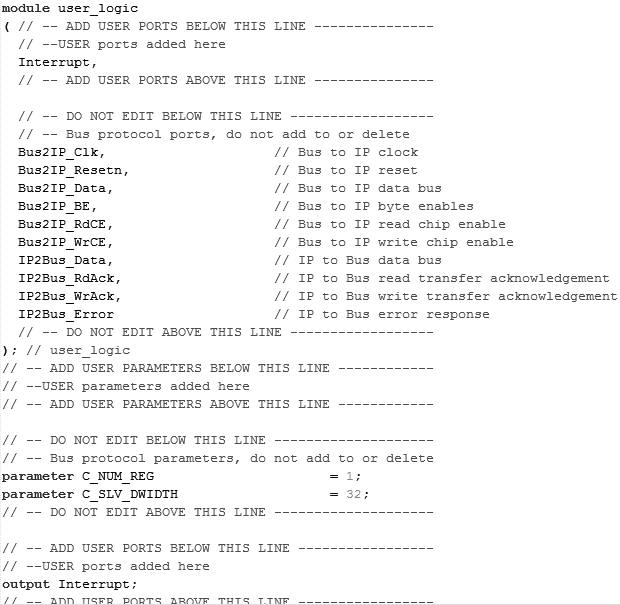
\includegraphics[width=.9\linewidth]{./apendices/interrupciones/img/int01}
				\end{center}
				\label{fig:int01}
				\caption{$ejemplo declarar puerto en user_logic$}
			\end{figure}
	\section{Modificaciones en el Software}
	
	Luego, este puerto de salida, debe ser declarado en el archivo ``$<nombre_ip_core>.vhd$'' que, como se 
	mencion� en la secci�n anterior es el que act�a de interfaz entre la l�gica del IP core y el sistema.

	En la declaraci�n del componente (Figura \ref{fig:int02}):
		\begin{figure}[H]
				\begin{center}
					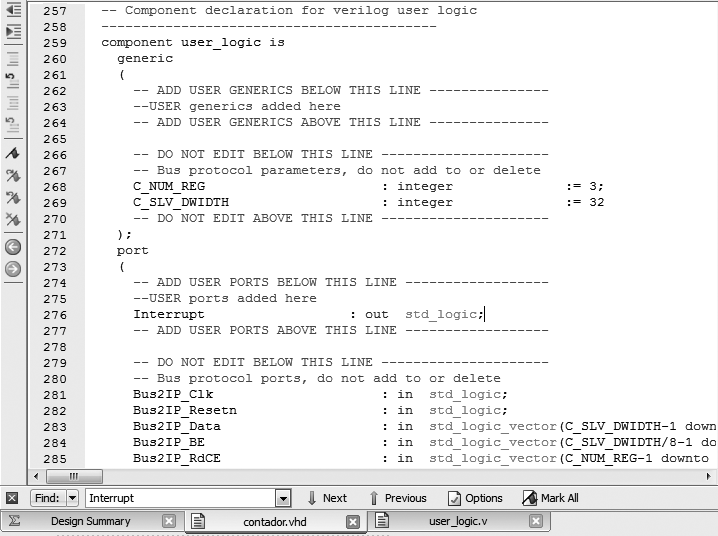
\includegraphics[width=.7\linewidth]{./apendices/interrupciones/img/int02}
				\end{center}
				\label{fig:int02}
				\caption{Agregado de puerto en  declaracion de componente}
			\end{figure}
			
	En la instanciaci�n del componente \emph{$user_logic$} (Figura \ref{fig:int02}):\\
		\begin{figure}[H]
				\begin{center}
					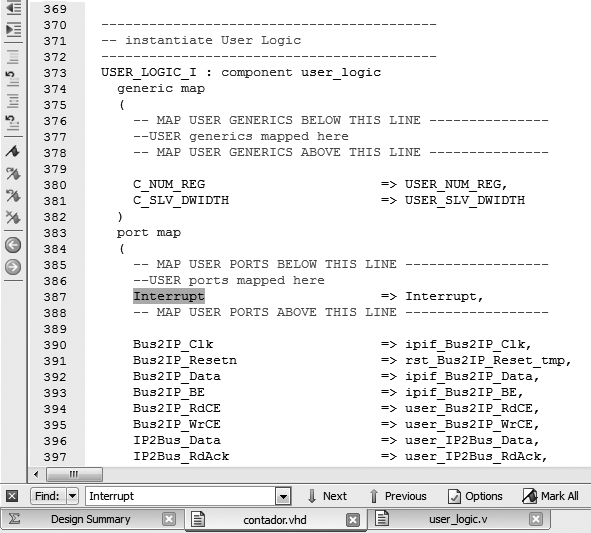
\includegraphics[width=.7\linewidth]{./apendices/interrupciones/img/int03}
				\end{center}
				\label{fig:int03}
				\caption{Agregado de puerto en implementacion del componente}
			\end{figure}	
	Y, finalmente en la declaraci�n de puertos (Figura \ref{fig:int04}):
		\begin{figure}[H]
				\begin{center}
					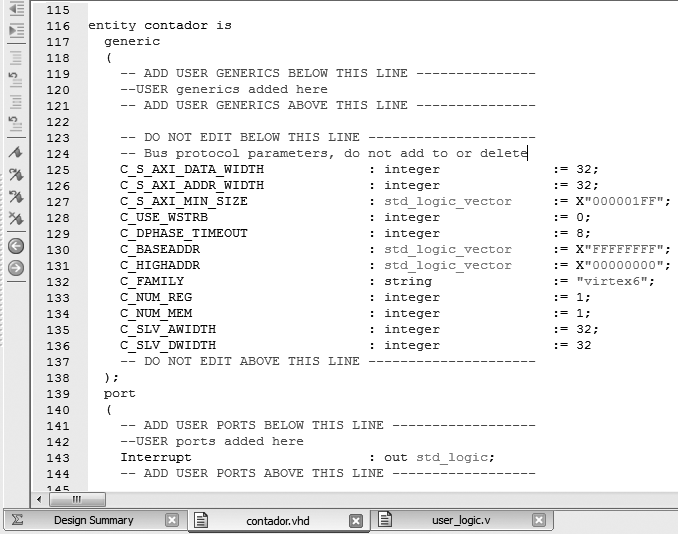
\includegraphics[width=.7\linewidth]{./apendices/interrupciones/img/int04}
				\end{center}
				\label{fig:int04}
				\caption{Agregado de puerto en la entidad}
			\end{figure}	
	Una vez que el puerto de interrupciones ha sido agregado, se debe conectar el mismo al controlador de 
	interrupciones del sistema.
	En XPS se tiene (Figura \ref{fig:int05}):
			\begin{figure}[H]
				\begin{center}
					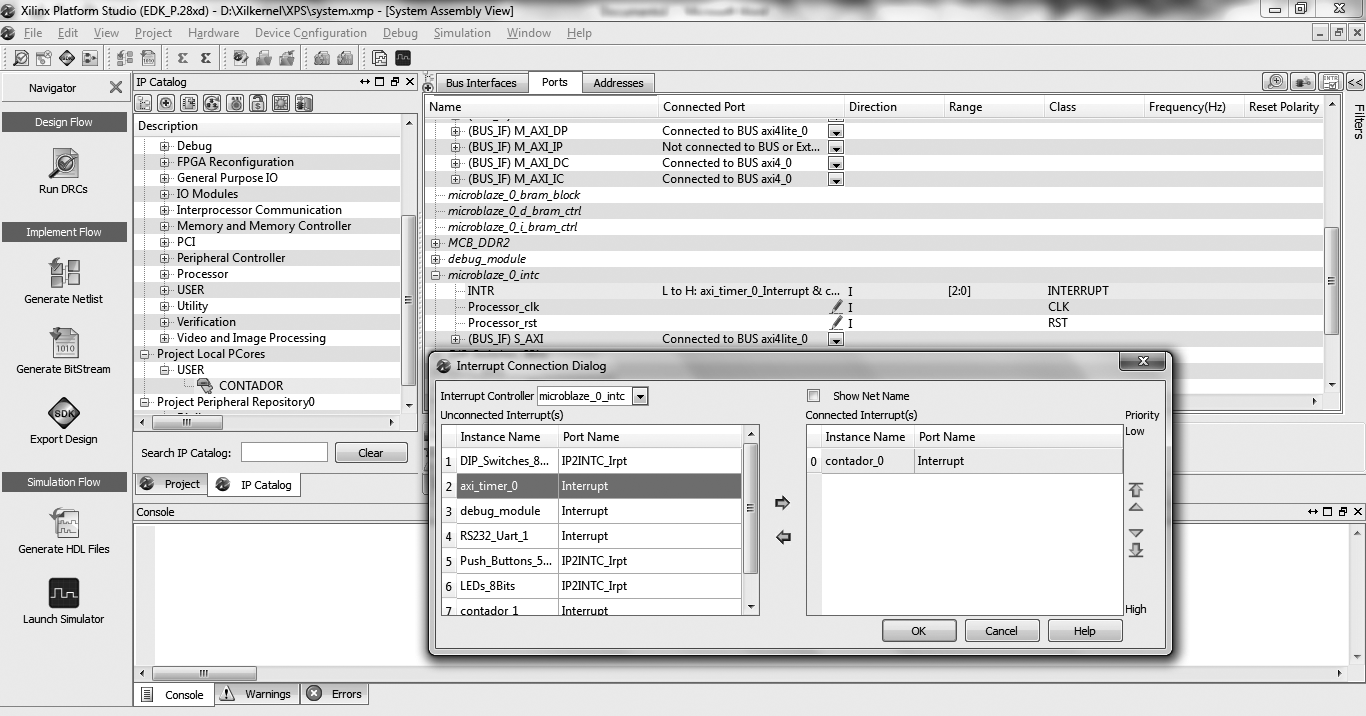
\includegraphics[width=.9\linewidth]{./apendices/interrupciones/img/int05}\\[2mm]
				\end{center}
				\label{fig:int05}
				\caption{Agregado en XPS}
			\end{figure}
	Una vez realizados los pasos anteriores, se debe sintetizar el proyecto y el IP core creado ya ser� 
	capaz de generar interrupciones.		
			
			
	\section{Modificaciones en el Software}
	
	Para habilitar las interrupciones se utiliza la API del Xilkernel. Esto se realiza mediante las 
	instrucciones ``register\_int\_handler'' y ``enable\_interrupt'':\\[1mm]

	register\_int\_handler($int\_id\_t\; intr\_id,void *handler),void *callback$);

	enable\_interrupt ($int\_id\_t\; intr\_id$);\\

	Estas funciones son para registrar el manejador de interrupciones y para habilitarlas respectivamente.
	Los par�metros de cada funci�n est�n definidos en la biblioteca ``xparameter.h'' incluida en el archivo 
	del programa. Estos par�metros son:
		\begin{itemize}
  			 \item \textbf{intr\_id:} Identificador de la Interrupci�n generalmente llamados \_INTERRUPT\_INTR.
  			 \item \textbf{handler:} Funci�n del tipo void que ser� llamada al producirse la interrupci�n.
  			 \item \textbf{callback:} Par�metro que se env�a a la funci�n para realizar una devoluci�n de datos.
		\end{itemize}
	Una vez realizado esto, la interrupci�n proveniente del IP core generado esta habilitada y ya se encuentra 
	registrado el manejador para su atenci�n (Figura \ref{fig:int07}).
	
		\begin{figure}[H]
				\begin{center}
					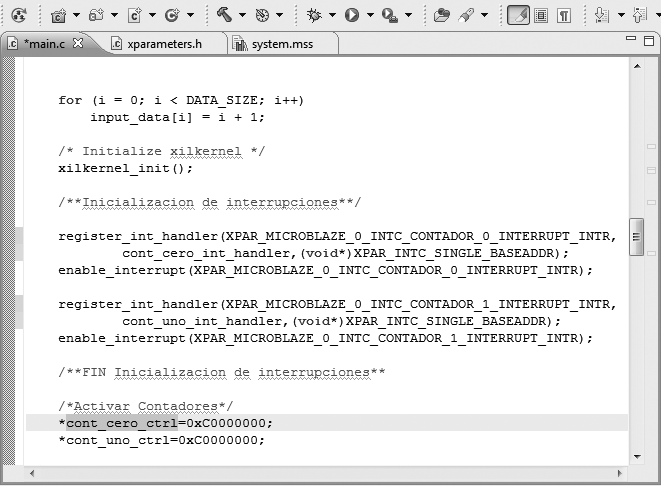
\includegraphics[width=.9\linewidth]{./apendices/interrupciones/img/int07}
				\end{center}
				\label{fig:int07}
				\caption{Agregado en SDK}
			\end{figure}
	